\documentclass[../main.tex]{subfiles}
\graphicspath{{\subfix{../imgs/}}}
\begin{document}

\chapter{Infraestructura desarrollada} \label{cap:infra}
Este capítulo aborda el diseño e implementación de la infraestructura software desarrollada para facilitar la programación de aplicaciones sobre drones. En primer lugar se explica el esquema seguido junto a las decisiones tomadas durante la fase de diseño. En segundo lugar, se presentan las diferentes herramientas desarrolladas y su implementación.

\section{Diseño} \label{section:infra-disenho}
La infraestructura ha sido diseñada desde el inicio teniendo en cuenta los objetivos y requisitos del proyecto. El esquema general del problema se presentan en la Figura \ref{fig:esq-gen}. Sobre el esquema se distinguen tres diferentes capas. En la parte inferior se encuentra la capa correspondiente a la aeronave, mientras que en la parte superior se encuentra el usuario, interesado en desarrollar una aplicación para controlar la aeronave. Entremedias se encuentra la herramienta a desarrollar, que se enfrenta al desafío de comunicarse con la aeronave, generalmente una tarea compleja, y de ofrecer al usuario una interfaz sencilla.

\begin{figure}[!ht]
 	\ffigbox[\FBwidth] {
 	    \caption[Esquema de capas de la infraestructura]{Esquema de capas de la infraestructura.}
        \label{fig:esq-gen}
    }
 	{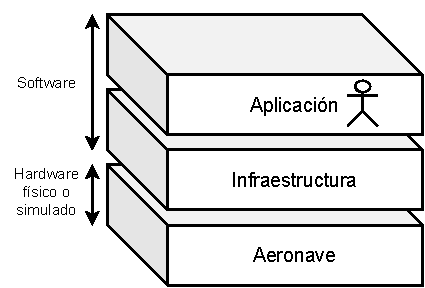
\includegraphics[width=0.65\textwidth]{04/esq-capas.pdf}}
\end{figure}

Para resolver el problema de la comunicación con la aeronave se ha decidido usar MAVROS, previamente presentado en el capítulo correspondiente al material utilizado. MAVROS establece una arquitectura de nodos, \emph{topics} y servicios que permiten comunicarse con la aeronave. Dichas herramientas se analizarán con profundidad en el Sección \ref{section:infra-wrapper}. \\
La interacción con el usuario se resuelve ofreciendo un paquete de ROS y fácilmente importables a Python. El paquete, llamado \emph{DroneWrapper}, ofrece una interfaz de programación al usuario que le permite controlar la aeronave ya sea física o simulada. El paquete posee una clase \emph{DroneWrapper}, de nombre igual al paquete, cuyos métodos proporcionan todo tipo de tareas para el trabajo con un multicóptero. \\
Así pues, el nuevo esquema que se obtiene con el diseño presentado hasta ahora se ilustra en la Figura \ref{fig:esq-bloq}.

\begin{figure}[!ht]
 	\ffigbox[1.3\FBwidth] {
 	    \caption[Diseño inicial de la infraestructura]{Diseño inicial de la infraestructura.}
        \label{fig:esq-bloq}
    }
 	{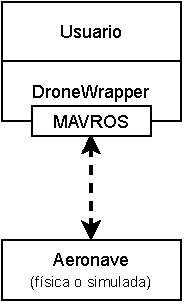
\includegraphics[width=0.35\textwidth]{04/esq-inic.pdf}}
\end{figure}

Es importante destacar que los objetivos de seguridad y robustez se ven cumplidos con MAVROS. La comunicación cuenta con la robustez de ROS, mientras la seguridad está presente al utilizar la versión 2.0 de MAVLink, la cual permite, entre otros aspectos de seguridad, el cifrado de los mensajes. 

Con este diseño se puede observar cómo la comunicación se realiza a través de MAVROS y dentro del paquete \emph{DroneWrapper} presentado. Según este último esquema, MAVROS tiene que poder entender y comunicarse con ambos extremos de la comunicación. \emph{DroneWrapper} no presenta problema ninguno, pues ha sido desarrollado para esta causa, pero la aeronave si puede suponer alguna dificultad. \\
MAVROS soporta los principales controladores de vuelo como PX4, presente en dos de las tres aeronaves utilizadas. Sin embargo, el Tello no posee soporte con MAVROS, tampoco con ROS, al ser un controlador privado. Para resolver dicho problema, se ha ideado y programado un controlador (o \emph{driver}) de comunicaciones que simula a MAVROS, llamado \emph{Tello Driver}.

\emph{Tello Driver} ofrece, de igual forma que hace MAVROS, una serie de nodos y servicios que permiten la comunicación con \emph{DroneWrapper}. Por otro lado, para comunicarse con la aeronave se utiliza el SDK oficial de Tello \cite{tello-sdk} que permite controlar la aeronave con mensajes especificado por el fabricante. \\
Siguiendo esta consideración, el esquema presentado se ve ligeramente modificado. El nuevo diseño se muestra en la Figura \ref{fig:esq-bloq2}.

\begin{figure}[!ht]
 	\ffigbox[1.3\FBwidth] {
 	    \caption[Diseño final de la infraestructura]{Diseño final de la infraestructura.}
        \label{fig:esq-bloq2}
    }
 	{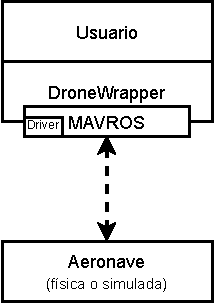
\includegraphics[width=0.35\textwidth]{04/esq-final.pdf}}
\end{figure}

\newpage
Así como el Tello necesita un \emph{driver} particular de comunicaciones, puede que otras aeronaves necesiten otro controlador de comunicaciones específico para hacer uso de la herramienta \emph{DroneWrapper}. \\
Otros elementos periféricos pueden también necesitar \emph{drivers} para encajar en la infraestructura dispuesta. Es el caso de la cámara utilizada (\emph{Victure}) en la aeronave de construcción propia. Para ofrecer las imágenes a través de la interfaz de \emph{DroneWrapper} se ha desarrollado también otro controlador, llamado \emph{Victure driver}. \\
Ambos \emph{drivers} se presentan al usuario en forma de paquetes de ROS, que el usuario puede incluir en la infraestructura software en función de sus necesidades. \\

\begin{figure}[!ht]
 	\ffigbox[\FBwidth] {
 	    \caption[Estructura modular de \emph{DroneWrapper}]{Estructura modular de \emph{DroneWrapper}.}
        \label{fig:esq-mod}
    }
 	{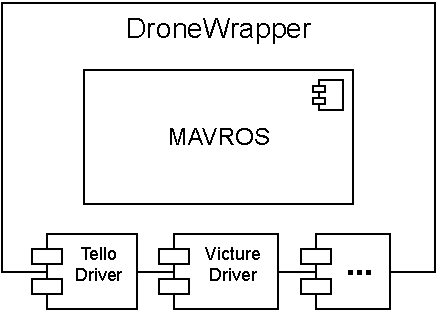
\includegraphics[width=0.65\textwidth]{04/esq-mod.pdf}}
\end{figure}

Antes de continuar con los detalles de implementación de los distintos paquetes es necesario discutir ciertos aspectos del diseño para una mejor comprensión del mismo. En primer lugar, se ha apostado por diseñar un paquete principal horizontal que congregue todos los aspectos comunes de la infraestructura. Sobre este recae una arquitectura modular (ver Fig. \ref{fig:esq-mod}), donde los distintos ``módulos'' (\emph{drivers} según se han introducido anteriormente) se pueden incluir según las necesidades de la aeronave o del usuario.

El diseño pretende reflejar a \emph{DroneWrapper} como una especie de driver genérico para multicópteros, independiente de los drivers concretos de bajo nivel de cada aeronave. Para aeronaves con controladores de vuelo PX4 y ArduPilot se utiliza MavLink y MAVROS directamente como elementos de comunicación. Asimismo, \emph{DroneWrapper} abstrae la funcionalidad fundamental como el control en velocidad, control en posición, así como los datos de los sensores habituales a bordo de las aeronaves.

El nombre elegido para el paquete (\emph{DroneWrapper}) hace referencia a la utilidad del mismo, ``envoltorio para drones''. Envoltorio pues envuelve a la aeronave y permite desarrollar sobre él aplicaciones de más alto nivel de abstracción obviando detalles cercanos al hardware.

\begin{figure}[!ht]
 	\ffigbox[\FBwidth] {
 	    \caption[Estructura de ``envoltorio'']{Estructura de ``envoltorio''.}
        \label{fig:esq-wrapper}
    }
 	{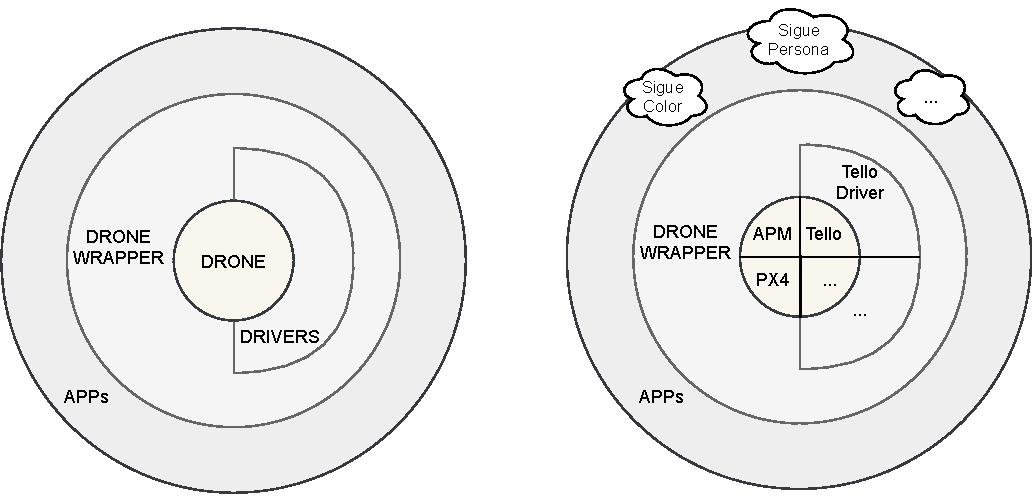
\includegraphics[width=\textwidth]{04/esq-env.pdf}}
\end{figure}

En las próximas secciones se analizarán los diferentes paquetes presentados, \emph{DroneWrapper}, \emph{Tello Driver} y \emph{Victure Driver}. Sobre ellos se explicará la estructura del paquete y su funcionamiento interno.

\section{Drone Wrapper} \label{section:infra-wrapper}
\emph{DroneWrapper} está organizado de forma similar a un paquete ROS tipo. El código se divide en diferentes carpetas en función de su utilidad. El directorio principal con el código fuente es \emph{src}. Otros carpetas contienen archivos de lanzamiento de ROS (\emph{launch}) o código de prueba (\emph{test}), entre otros. Los archivos \emph{launch} solo tienen uso con la aeronave simulada pues permiten lanzar la simulación de PX4 junto a MAVROS en Gazebo. \\
\emph{DroneWrapper} se enmarca dentro de un meta-paquete junto a otros paquetes, como por ejemplo \emph{Tello Driver}. El meta-paquete congrega los útiles para drones de JdeRobot. \\
El código se encuentra disponible en abierto en el repositorio \emph{drones/drone\_wrapper} \footnote{\url{https://github.com/JdeRobot/drones/tree/melodic-devel/drone_wrapper}} de JdeRobot. En este momento, el paquete dispone de aproximadamente 1000 líneas de código entre los diferentes archivos, de las cuales casi 700 son de código fuente.

\emph{DroneWrapper}, al igual que todo paquete de \emph{ROS}, utiliza una serie de herramientas para mantener la comunicación. Estas herramientas son los nodos, \emph{topics}, servicios y parámetros. Los nodos son procesos, los \emph{topics} canales de comunicación entre dos nodos, los servicios son métodos de comunicación por petición y los parámetros sirve para almacenar y manipular datos. \\
El esquema en ejecución de \emph{DroneWrapper} se muestra en la Figura \ref{fig:esq-nodos}. El grafo muestra los \emph{topics} o canales de intercambio de mensajes. A ambos lados se sitúan los diferentes nodos. Por un lado, MAVROS (\lstinline{/mavros} en la figura), quien realiza la comunicación con la aeronave, y por otro lado, \emph{DroneWrapper} (\lstinline{/drone}), accesible al usuario. El nodo de MAVROS es el estándar del paquete, que se ejecuta tal como indica su documentación.

% Posición original de FIG Grafo de nodos

\begin{table}[H]
	\ttabbox[\FBwidth]
	{\caption{\emph{Topics} presentes en \emph{DroneWrapper}} \label{tab:topics}}
	{\begin{tabular}{|c|c|c|}
		\hline
		\multicolumn{2}{|c|}{\textbf{\emph{topic}}} & \textbf{Tipo de mensaje} \\
		\hline
		\multirow{7}{*}{Public.} & \lstinline{/mavros/state} & \lstinline{mavros_msgs/State()} \\
		\cline{2-3}
		 & \lstinline{/mavros/extended_state} & \lstinline{mavros_msgs/ExtendedState()} \\
		\cline{2-3}
		 & \lstinline{/mavros/local_position/pose} & \lstinline{geometry_msgs/PoseStamped()} \\
		\cline{2-3}
		 & \lstinline{/mavros/local_position/velocity_body} & \lstinline{geometry_msgs/TwistStamped()} \\
		\cline{2-3}
		 & \lstinline{/mavros/global_position/global} & \lstinline{sensor_msgs/NavSatFix()} \\
		\cline{2-3}
		 & \lstinline{/mavros/battery} & \lstinline{sensor_msgs/BatteryState()} \\
		\cline{2-3}
		 & \lstinline{/iris/cam_frontal/image_raw} & \lstinline{sensor_msgs/Image()} \\
		\cline{2-3}
		 & \lstinline{/iris/cam_ventral/image_raw} & \lstinline{sensor_msgs/Image()} \\
		\hline
		Subscr. & \lstinline{/mavros/setpoint_raw/local} & \lstinline{mavros_msgs/PositionTarget()} \\
		\hline
		\multicolumn{3}{l}{Fuente: ROS Wiki}
	\end{tabular}}
\end{table}

Sobre los \emph{topics} distinguimos dos grupos, los publicadores de mensajes y los receptores o subscriptores de mensajes. Nótese que cada \emph{topic} es publicador o subscriptor en función del nodo en cuestión en el que se fije la atención. La clasificación se realiza sobre el nodo de \emph{DroneWrapper} pues el paquete que se pretende explicar en esta sección. \\
Entre los publicadores de mensajes (y sobre los que se subscribe la aplicación) se encuentran 8 \emph{topics}, los cuales envían información de estado de la aeronave, como la posición o datos de la batería, junto a las imágenes de las cámaras (en este caso de los \emph{plugins} al encontrarnos con una aeronave simulada). \\
Por otro lado, solo existe un subscriptor (al que la aplicación le envía mensajes), el cual se encarga de enviar comandos y órdenes de actuación a la aeronave. En la Tabla \ref{tab:topics} se muestran los \emph{topics} utilizados junto al tipo de mensaje usado.

\begin{figure}[!ht]
 	\ffigbox[\FBwidth] {
 	    \caption[Grafo de nodos y \emph{topics} de \emph{DroneWrapper}]{Grafo de nodos y \emph{topics} de \emph{DroneWrapper}.}
        \label{fig:esq-nodos}
    }
 	{\includesvg[width=0.87\textwidth]{04/rosgraph.svg}}
\end{figure}
\clearpage

El control sobre la aeronave se realiza a través del \emph{topic} \lstinline{/mavros/setpoint_raw/local}. Para entender correctamente su funcionamiento, es necesario analizar el tipo de mensaje \lstinline{mavros_msgs/PositionTarget()}. El Código \ref{lst:positiontarget} muestra la definición del mensaje. \\
Es importante destacar que para los autopilotos puedan responder correctamente a dichos mensajes es necesario que se encuentren en un modo de vuelo concreto. En el caso de PX4, este modo de vuelo es \lstinline{OFFBOARD}.

\lstinputlisting[caption={Definición del mensaje \lstinline{mavros_msgs/PositionTarget()}}, language=xml, captionpos=b, label={lst:positiontarget}]{code/positiontarget.msg}

El mensaje \lstinline{PositionTarget()} permite el uso de diferentes marcos de coordenadas (\lstinline{coordinate_frame}). La aplicación utiliza siempre el mismo eje, \lstinline{FRAME_BODY_NED (8)}, que pese al nombre se comporta como un eje local, fijo al punto de despegue, y con orientación Norte-Este-Abajo (NED, \emph{North-East-Down}).

Este mensaje permite también diferentes tipos de control, en posición, en velocidad, en aceleración, en fuerza y con controles mixtos, a través de los últimos campos del mensaje. Dichos controles se seleccionan en función de la máscara \lstinline{type_mask} activa. Nótese que no todas las máscaras son válidas.
\emph{DroneWrapper} soporta tres tipos de control, en posición, en velocidad y mixto basado en un control en velocidad con altura de vuelo fija. Las máscaras utilizadas se ilustran en la Tabla \ref{tab:mask}.

\begin{table}[H]
	\ttabbox[\FBwidth]
	{\caption{Máscaras de control utilizadas por \emph{DroneWrapper}} \label{tab:mask}}
	{\begin{tabular}{|c|c|c|}
		\hline
		\textbf{Control} & \textbf{Máscara} & \textbf{Campos activos} \\
		\hline
		Posición & 3064 & \lstinline{x y z yaw}  \\
		\hline
        Velocidad & 1991 & \lstinline{vx vy vz yaw_rate} \\
        \hline
        Mixto & 1987 & \lstinline{vx vy vz z yaw_rate} \\
        \hline
		\multicolumn{3}{l}{Fuente: Elaboración propia}
	\end{tabular}}
\end{table}

Además de \emph{topics}, la aplicación hace uso de servicios y parámetros. Los servicios son utilizados para lanzar solicitudes a la aeronave de diversa índole. Estas solicitudes se encargan del armado de la aeronave, del aterrizaje, del cambio de modo y de la manipulación de los parámetros. La Tabla \ref{tab:serv} recoge los servicios utilizados por \emph{DroneWrapper}.

\begin{table}[ht]
	\ttabbox[\FBwidth]
	{\caption{Servicios presentes en \emph{DroneWrapper}} \label{tab:serv}}
	{\begin{tabular}{|c|c|}
		\hline
		\textbf{Servicio} & \textbf{Tipo de servicio} \\
		\hline
		\lstinline{/mavros/cmd/arming} & \lstinline{mavros_msgs/CommandBool()} \\
		\hline
		\lstinline{/mavros/cmd/land} & \lstinline{mavros_msgs/CommandTOL()} \\
		\hline
		\lstinline{/mavros/set_mode} & \lstinline{mavros_msgs/SetMode()} \\
		\hline
		\lstinline{/mavros/param/set} & \lstinline{mavros_msgs/ParamSet()} \\
		\hline
		\lstinline{/mavros/param/get} & \lstinline{mavros_msgs/ParamGet()} \\
		\hline
		\multicolumn{2}{l}{Fuente: ROS Wiki}
	\end{tabular}}
\end{table}

Finalmente, los parámetros utilizados por la aplicación son solamente uno, aunque MAVROS utiliza múltiples internamente para poder realizar sus tareas. El parámetro usado por \emph{DroneWrapper} es \lstinline{drone_model}. Como su nombre indica sirve para representar el modelo de la aeronave, muy útil para manejar sensores y otros elementos que difieren entre aeronaves. En simulación, por ejemplo, el valor del parámetro es \lstinline{iris}, correspondiente al modelo de la aeronave simulada.

Hasta ahora se ha presentado el funcionamiento interno y más próximo a la aeronave de la infraestructura. A continuación, se explicará el otro extremo, más cercano al usuario. Ya se ha adelantado que \emph{DroneWrapper} se presenta al usuario como un paquete importable en Python y con una serie de métodos (API) que permiten operar con la aeronave.

\lstinputlisting[caption={Caso de uso simple de \emph{DroneWrapper}}, language=python, captionpos=b, label={lst:dw-simple}]{code/dw-simple.py}

Un caso de uso sencillo se presenta en el Código \ref{lst:dw-simple}. En él, se crea, en primer lugar, un objeto que representa al dron y que da acceso a todas las funcionalidades presentes en el paquete. A continuación, se le ordena despegar y tras ello, el dron da vueltas sobre sí mismo durante varios segundos. Finalmente el dron aterriza en la posición actual. Cabe destacar que el esquema de nodos presentado anteriormente (Fig. \ref{fig:esq-nodos}) se ha obtenido con la aeronave simulada y el código ahora mostrado.

Finalmente, la API presente en \emph{DroneWrapper} se muestra en la Tabla \ref{tab:api}. En ella se recogen los métodos que permiten obtener información sobre los sensores y estado de la aeronave, los métodos para controlar a la aeronave y los métodos para obtener las imágenes de las cámaras de la aeronave.

\begin{table}[H]
	\ttabbox[\FBwidth]
	{\caption{\emph{DroneWrapper} API} \label{tab:api}}
	{\begin{tabular}{|c|c|c|}
		\hline
		\multicolumn{2}{|c|}{\textbf{API}} & \textbf{Descripción} \\
		\hline
		 & \multirow{2}{*}{\lstinline{[x, y, z] = get_position()}} & Devuelve la posición \\
		                                                         & & de la aeronave (m) \\
		\cline{2-3}
		 & \multirow{2}{*}{\lstinline{[vx, vy, vz] = get_velocity()}} & Devuelve la velocidad \\
		                                                            & & de la aeronave (m/s) \\
		\cline{2-3}
		 & \multirow{2}{*}{\lstinline{rate = get_yaw_rate()}} & Devuelve la velocidad \\
		                                                   &  & de guiñada de la aeronave (rad/s) \\
		\cline{2-3}
		 & \multirow{2}{*}{\lstinline{[r, p, y] = get_orientation()}} & Devuelve la orientación \\
		Sensores &                                                    & de la aeronave (rad) \\
		\cline{2-3}
		y estado & \multirow{2}{*}{\lstinline{r = get_roll()}} & Devuelve el ángulo de alabeo \\
		                                                    &  & de la aeronave (rad) \\
		\cline{2-3}
		 & \multirow{2}{*}{\lstinline{p = get_pitch()}} & Devuelve el ángulo de cabeceo \\
		                                              & & de la aeronave (rad)  \\
		\cline{2-3}
		 & \multirow{2}{*}{\lstinline{y = get_yaw()}} & Devuelve el ángulo de guiñada \\
		                                            & & de la aeronave (rad) \\
		\cline{2-3}
		 & \multirow{2}{*}{\lstinline{s = get_landed_state()}} & Devuelve si la aeronave está en \\
		                                            & & tierra (1), volando (2) o aterrizando (4) \\
		\hline
		\multirow{8}{*}{Control} & \lstinline{takeoff(h)} & Despegue a altura \lstinline{h} (m) \\
		\cline{2-3}
		& \lstinline{land()} & Aterrizaje en posición actual \\
		\cline{2-3}
		 & \multirow{2}{*}{\lstinline{set_cmd_pos(x, y, z, yaw)}} & Control en posición x, y, z (m) \\
		                                                        & & y guiñada (rad) \\
		\cline{2-3}
		 & \multirow{2}{*}{\lstinline{set_cmd_vel(vx, vy, vz, vyaw)} } & Control en velocidad vx, vy, vz (m/s)\\
		 & & y guiñada (rad/s) \\
		\cline{2-3}
		 & \multirow{2}{*}{\lstinline{set_cmd_mix(vx, vy, z, vyaw)}} & Control mixto vx, vy (m/s), \\
		 & & z (m) y guiñada (rad/s) \\
		\hline
		\multirow{2}{*}{Cámaras} & \multirow{1}{*}{\lstinline{img = get_frontal_image()}} & Devuelve la imagen de la cám. frontal \\
		\cline{2-3}
		& \multirow{1}{*}{\lstinline{img = get_ventral_image()}} & Devuelve la imagen de la cám. ventral \\
		\hline
		\multicolumn{3}{l}{Fuente: Elaboración propia}
	\end{tabular}}
\end{table}

\newpage
\section{Tello Driver} \label{section:infra-tello}
Al igual que el paquete anterior, \emph{Tello Driver} es un paquete ROS y está organizado de tal forma. En su directorio raíz se encuentran diferentes carpetas que reúnen el código en función de su propósito. En el directorio \emph{src} está el código fuente, en el directorio \emph{launch} se hallan archivos de lanzamiento, en el directorio \emph{test} hay diferentes códigos de prueba y en el directorio \emph{scripts} se encuentran varios ejecutables que permiten realizar acciones como aterrizar, despegar o una desconexión rápida de emergencia. \\
Al igual que \emph{DroneWrapper}, el paquete \emph{Tello Driver} pertenece al meta-paquete de drones de JdeRobot. \\
El código se encuentra disponible en abierto en el repositorio \emph{drones/tello\_driver} \footnote{\url{https://github.com/JdeRobot/drones/tree/melodic-devel/tello_driver}} de JdeRobot. En este momento, el paquete dispone de más 900 líneas de código entre los diferentes archivos, de las cuales casi 600 son de código fuente.

\emph{Tello Driver} posee dos principales tareas, comunicarse con \emph{DroneWrapper} y con la aeronave Tello. Para mostrar de forma clara su implementación, ambas partes se presentarán por separado, aunque no tengan sentido una parte en ausencia de la otra.

En la sección de diseño se ha adelantado el uso del Tello SDK para la comunicación con la aeronave física. Siguiendo las indicaciones para su uso, el \emph{driver} hace uso de una serie de \emph{sockets} e hilos para realizar la comunicación. La arquitectura de la comunicación se muestra en la Figura \ref{fig:esq-com}.

\begin{figure}[!ht]
 	\ffigbox[\FBwidth] {
 	    \caption[Esquema de comunicaciones de \emph{Tello Driver}]{Esquema de comunicaciones de \emph{Tello Driver}.}
        \label{fig:esq-com}
    }
 	{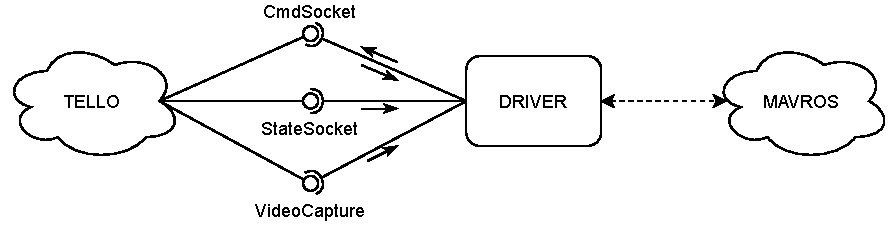
\includegraphics[width=0.95\textwidth]{04/tellodriver.pdf}}
\end{figure}

El \emph{driver} posee tres \emph{sockets}. El primero de ellos, \emph{CmdSocket} usado para el envío de comandos y para recibir la respuesta de los comandos. Es el único de los tres \emph{sockets} bidireccional. El segundo de los \emph{sockets}, \emph{StateSocket}, es utilizado para recibir la información de estado de la aeronave. Finalmente, el \emph{socket} \emph{VideoCapture} se encarga de recibir las imágenes envíadas desde el Tello.

Toda la información recibida se maneja desde tres distintos manejadores de mensajes (\emph{handlers}), en hilos secundarios, que se encargan de escuchar por los tres respectivos \emph{sockets} la información recibida. En cambio, los comandos enviados a la aeronave se atienden a través del hilo principal del \emph{driver}. Los detalles de la arquitectura de la comunicación se resumen en la Tabla \ref{tab:com}.

\begin{table}[H]
	\ttabbox[\FBwidth]
	{\caption{Máscaras de control utilizadas por \emph{Tello Driver}} \label{tab:com}}
	{\begin{tabular}{|c|c|c|c|}
		\hline
		\textbf{\emph{Socket}} & \textbf{Dirección} & \textbf{Hilo} & \textbf{Uso} \\
		\hline
		\multirow{2}{*}{\emph{CmdSocket}} & \lstinline{192.168.10.1:8889} & Hilo ppal. & Envío de comandos \\
		\cline{2-4}
         & \lstinline{0.0.0.0:9000} & Response handler & Respuesta de comandos \\
		\hline
        \emph{StateSocket} & \lstinline{0.0.0.0:8890} & State handler & Recepción datos de estado \\
        \hline
        \emph{VideoCapture} & \lstinline{0.0.0.0:11111} & Video handler & Recepción de vídeo \\
        \hline
		\multicolumn{4}{l}{Fuente: Tello SDK. Elaboración propia}
	\end{tabular}}
\end{table}

El \emph{driver} tiene por otro lado la comunicación con MAVROS (ver Fig. \ref{fig:esq-com}). De forma similar a \emph{DroneWrapper}, la comunicación se realiza a través de ocho \emph{topics}, siete publicadores y un subscriptor, y seis servicios. La comunicación es casi idéntica a la presentada con \emph{DroneWrapper}, pues se trata de imitar el comportamiento estándar de MAVROS para que la aplicación no note diferencia entre distintos drones. Como únicas diferencias se encuentran un nuevo servicio para despegar, aunque en la práctica no se utiliza con \emph{DroneWrapper} (sí con algún ejecutable del paquete), y la ausencia de uno de los dos publicadores de imágenes, pues el Tello solo posee una cámara. La Tabla \ref{tab:arq-ros} recoge de forma resumida la arquitectura de \emph{ROS} utilizada. Asimismo, la Figura \ref{fig:esq-nodos-tello} ilustra el grafo de nodos y \emph{topics} utilizado.

\begin{table}[H]
	\ttabbox[\FBwidth]
	{\caption{Arquitectura ROS de \emph{Tello Driver}} \label{tab:arq-ros}}
	{\begin{tabular}{|c|c|c|}
		\hline
		\multicolumn{2}{|c|}{\textbf{\emph{topic}}} & \textbf{Tipo de mensaje} \\
		\hline
		\multirow{6}{*}{Public.} & \lstinline{/mavros/state} & \lstinline{mavros_msgs/State()} \\
		\cline{2-3}
		 & \lstinline{/mavros/extended_state} & \lstinline{mavros_msgs/ExtendedState()} \\
		\cline{2-3}
		 & \lstinline{/mavros/local_position/pose} & \lstinline{geometry_msgs/PoseStamped()} \\
		\cline{2-3}
		 & \lstinline{/mavros/local_position/velocity_body} & \lstinline{geometry_msgs/TwistStamped()} \\
		\cline{2-3}
		 & \lstinline{/mavros/global_position/global} & \lstinline{sensor_msgs/NavSatFix()} \\
		\cline{2-3}
		 & \lstinline{/mavros/battery} & \lstinline{sensor_msgs/BatteryState()} \\
		\cline{2-3}
		 & \lstinline{/tello/cam_frontal/image_raw} & \lstinline{sensor_msgs/Image()} \\
		\hline
		Subscr. & \lstinline{/mavros/setpoint_raw/local} & \lstinline{mavros_msgs/PositionTarget()} \\
		\hline
		\multicolumn{3}{c}{} \\
		\hline
		\multicolumn{2}{|c|}{\textbf{Servicio}} & \textbf{Tipo de servicio} \\
		\hline
		\multicolumn{2}{|c|}{\lstinline{/mavros/cmd/arming}} & \lstinline{mavros_msgs/CommandBool()} \\
		\hline
		\multicolumn{2}{|c|}{\lstinline{/mavros/cmd/takeoff}} & \lstinline{mavros_msgs/CommandTOL()} \\
		\hline
		\multicolumn{2}{|c|}{\lstinline{/mavros/cmd/land}} & \lstinline{mavros_msgs/CommandTOL()} \\
		\hline
		\multicolumn{2}{|c|}{\lstinline{/mavros/set_mode}} & \lstinline{mavros_msgs/SetMode()} \\
		\hline
		\multicolumn{2}{|c|}{\lstinline{/mavros/param/set}} & \lstinline{mavros_msgs/ParamSet()} \\
		\hline
		\multicolumn{2}{|c|}{\lstinline{/mavros/param/get}} & \lstinline{mavros_msgs/ParamGet()} \\
		\hline
		\multicolumn{3}{l}{Fuente: ROS Wiki}
	\end{tabular}}
\end{table}

\begin{figure}[!ht]
 	\ffigbox[\FBwidth] {
 	    \caption[Grafo de nodos y \emph{topics} de \emph{Tello Driver}]{Grafo de nodos y \emph{topics} de \emph{Tello Driver}.}
        \label{fig:esq-nodos-tello}
    }
 	{\includesvg[width=\textwidth]{04/rosgraph-tello.svg}}
\end{figure}

\newpage
Tras explicar ambos extremos del \emph{driver}, falta por explicar la parte intermedia que convierte los mensajes y servicios de ROS en un lenguaje de mensajes entendidos por el Tello SDK y viceversa. El envío de comandos de actuación se realiza enviando una cadena de texto a través del \emph{socket} previamente mostrado. En función del contenido de la cadena de texto, la aeronave interpreta una orden u otra. Son muchas las órdenes aceptadas en el Tello SDK, la Tabla \ref{tab:cmd-sdk} solamente recoge las utilizadas por el \emph{driver}.

El \emph{driver} se encarga de traducir los comandos recibidos por el \emph{topic} subscriptor y a través de los servicios en los distintos mensajes de la tabla, para que la aeronave realice la tarea ordenada. La respuesta al comando se obtiene por uno de los \emph{handlers} y se notifica a través de MAVROS.

\begin{table}[H]
	\ttabbox[\FBwidth]
	{\caption{Comandos usados por \emph{Tello Driver}} \label{tab:cmd-sdk}}
	{\begin{tabular}{|c|c|c|}
		\hline
		\textbf{Comando} & \textbf{Descripción} & \textbf{Posible respuesta} \\
		\hline
        \lstinline{command} & Entrada al modo SDK & \lstinline{ok} / \lstinline{error} \\
		\hline
        \lstinline{streamon} & Habilitar transmisión de vídeo & \lstinline{ok} / \lstinline{error} \\
		\hline
        \lstinline{streamoff} & Deshabilitar transmisión de vídeo & \lstinline{ok} / \lstinline{error} \\
		\hline
        \lstinline{emergency} & Parada de motores de emergencia & \lstinline{ok} / \lstinline{error} \\
		\hline
        \lstinline{takeoff} & Despegue & \lstinline{ok} / \lstinline{error} \\
		\hline
        \lstinline{land} & Aterrizaje & \lstinline{ok} / \lstinline{error} \\
		\hline
        \lstinline{forward x} & Avanza \lstinline{x} cm & \lstinline{ok} / \lstinline{error} \\
		\hline
        \lstinline{back x} & Retrocede \lstinline{x} cm & \lstinline{ok} / \lstinline{error} \\
		\hline
        \lstinline{left x} & Izquierda \lstinline{x} cm & \lstinline{ok} / \lstinline{error} \\
		\hline
        \lstinline{right x} & Derecha \lstinline{x} cm & \lstinline{ok} / \lstinline{error} \\
		\hline
        \lstinline{up x} & Suba \lstinline{x} cm & \lstinline{ok} / \lstinline{error} \\
		\hline
        \lstinline{down x} & Baje \lstinline{x} cm & \lstinline{ok} / \lstinline{error} \\
		\hline
        \lstinline{cw x} & Rota \lstinline{x} grados (horario) & \lstinline{ok} / \lstinline{error} \\
		\hline
        \lstinline{ccw x} & Rota \lstinline{x} grados (anti-horario) & \lstinline{ok} / \lstinline{error} \\
		\hline
        \multirow{6}{*}{\lstinline{rc a b c d}} & Control remoto (cm/s) & \multirow{6}{*}{\lstinline{ok} / \lstinline{error}} \\
         & & \\
         & \lstinline{a} derecha/izquierda (-100,100) & \\
         & \lstinline{b} adelante/atrás (-100,100) & \\
         & \lstinline{c} arriba/abajo (-100,100) & \\
         & \lstinline{d} guiñada (-100,100) & \\
		\hline
        \lstinline{battery?} & Obtén la batería restante & \lstinline{x} (0-100) \\
		\hline
		\multicolumn{3}{l}{Fuente: Tello SDK}
	\end{tabular}}
\end{table}

Por otro lado, el estado de la aeronave se recibe a través del \emph{StateSocket} en una cadena de texto con aspecto: \lstinline{dato:valor;dato2:valor2;....;\r\n}. El conjunto de datos enviados por el Tello se muestra en la Tabla \ref{tab:data-sdk} por orden de aparición en la cadena de texto. Dichos valores se procesan en el \emph{driver}, se encapsulan en los diferentes mensajes de ROS y se envían a través de los distintos \emph{topics}.

\begin{table}[H]
	\ttabbox[\FBwidth]
	{\caption{Información recibida por \emph{Tello Driver}} \label{tab:data-sdk}}
	{\begin{tabular}{|c|c|}
		\hline
		\textbf{Información} & \textbf{Descripción} \\
		\hline
        \lstinline{pitch} & Ángulo de cabeceo (grados) \\
		\hline
        \lstinline{roll} & Ángulo de alabeo (grados) \\
		\hline
        \lstinline{yaw} & Ángulo de guiñada (grados) \\
		\hline
        \lstinline{vgx} & Velocidad en eje x (cm/s) \\
		\hline
        \lstinline{vgy} & Velocidad en eje y (cm/s) \\
		\hline
        \lstinline{vgz} & Velocidad en eje z (cm/s) \\
		\hline
        \lstinline{templ} & Temperatura mínima (Cº) \\
		\hline
        \lstinline{temph} & Temperatura máxima (Cº) \\
		\hline
        \lstinline{tof} & Distancia recorrida desde despegue (cm) \\
		\hline
        \lstinline{h} & Altura (cm) \\
		\hline
        \lstinline{bat} & Nivel de batería (\%) \\
		\hline
        \lstinline{baro} & Medición barométrica (cm) \\
		\hline
        \lstinline{time} & Tiempo de vuelo (s) \\
		\hline
        \lstinline{agx} & Aceleración en eje x (cm/s$^2$) \\
		\hline
        \lstinline{agy} & Aceleración en eje y (cm/s$^2$) \\
		\hline
        \lstinline{agz} & Aceleración en eje z (cm/s$^2$) \\
		\hline
		\multicolumn{2}{l}{Fuente: Tello SDK}
	\end{tabular}}
\end{table}

Finalmente, a través del \emph{VideoCapture} se reciben los distintos fotogramas que se retransmiten a través del \emph{topic} preparado para ello.

\section{Victure Driver} \label{section:infra-victure}
El \emph{driver} para la cámara integrado en la infraestructura, \emph{Victure driver}, posee al igual que los dos paquete anteriores una estructura de paquete de ROS. Sobre el directorio principal se encuentra una carpeta con el código fuente (\emph{src}), una carpeta con código para probar el \emph{driver} (\emph{test}) y una carpeta con ficheros de lanzamiento (\emph{launch}). \\
El código se encuentra disponible en el repositorio \emph{RoboticsLabURJC/2021-tfm-pedro-arias} \footnote{\url{https://github.com/RoboticsLabURJC/2021-tfm-pedro-arias/tree/main/victure_driver}} de forma pública. En este momento, el paquete dispone de aproximadamente 300 líneas de código entre los diferentes archivos.

La estructura ROS es muy simple. El \emph{driver} se compone de un nodo (\lstinline{victure_cam}) que lee imágenes de la cámara y las envía a través de un \emph{topic} (\lstinline{victure_cam/image_raw}). El código del \emph{driver} se muestra en el Código \ref{lst:victure}. 

\begin{figure}[!ht]
 	\ffigbox[\FBwidth] {
 	    \caption[Grafo de nodos y \emph{topics} de \emph{Victure Driver}]{Grafo de nodos y \emph{topics} de \emph{Victure Driver}.}
        \label{fig:esq-nodos-vict}
    }
 	{\includesvg[width=0.95\textwidth]{04/rosgraph-vict.svg}}
\end{figure}

\newpage
\lstinputlisting[caption={\emph{Victure Driver}}, language=python, captionpos=b, label={lst:victure}]{code/video_bridge.py}

Finalmente, el grafo de nodos del \emph{driver} se muestra en la Figura \ref{fig:esq-nodos-vict}. La figura recoge el nodo principal junto a un nodo de prueba (\emph{test}), que se encarga de leer sobre el \emph{topic} y mostrar por pantalla la imagen recibida (ver Figura \ref{fig:img-vict}).

\begin{figure}[!ht]
 	\ffigbox[\FBwidth] {
 	    \caption[Imagen obtenida por el \emph{Victure driver}]{Imagen obtenida por el \emph{Victure driver}.}
        \label{fig:img-vict}
    }
 	{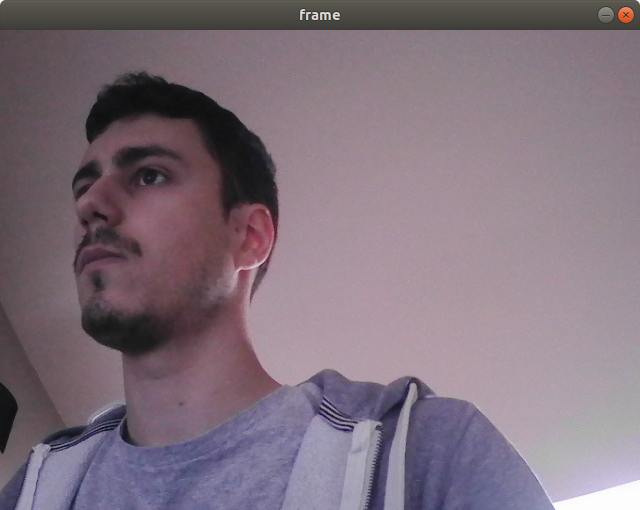
\includegraphics[width=0.6\textwidth]{04/vict-img.png}}
\end{figure}

\end{document}

